\subsection{Trajectory Analysis}\label{sec:trajectory}

Though the completion time analysis indicates that Hydra / 3D headtracked
combination results in the fastest mean completion time, it possible to derive
insights from visualizing the data itself, in aggregate and on a per subject
basis.  These analyses are subjective.  In the following, all input data were
normalized so that the start target is at the origin and the end target lies
on the positive $x$-axis.

\figref{fig:compressedtracks} shows the tracks for each input/output
combination. Each path is data from a trial; green indicates a trial
completion time of less than 10 seconds and red is over 10 seconds.  Each
point was rotated around the $x$-axis so that it lies on the XY plane,
discarding Z information while minimizing angular distortion.

\begin{figure}
    \centering
    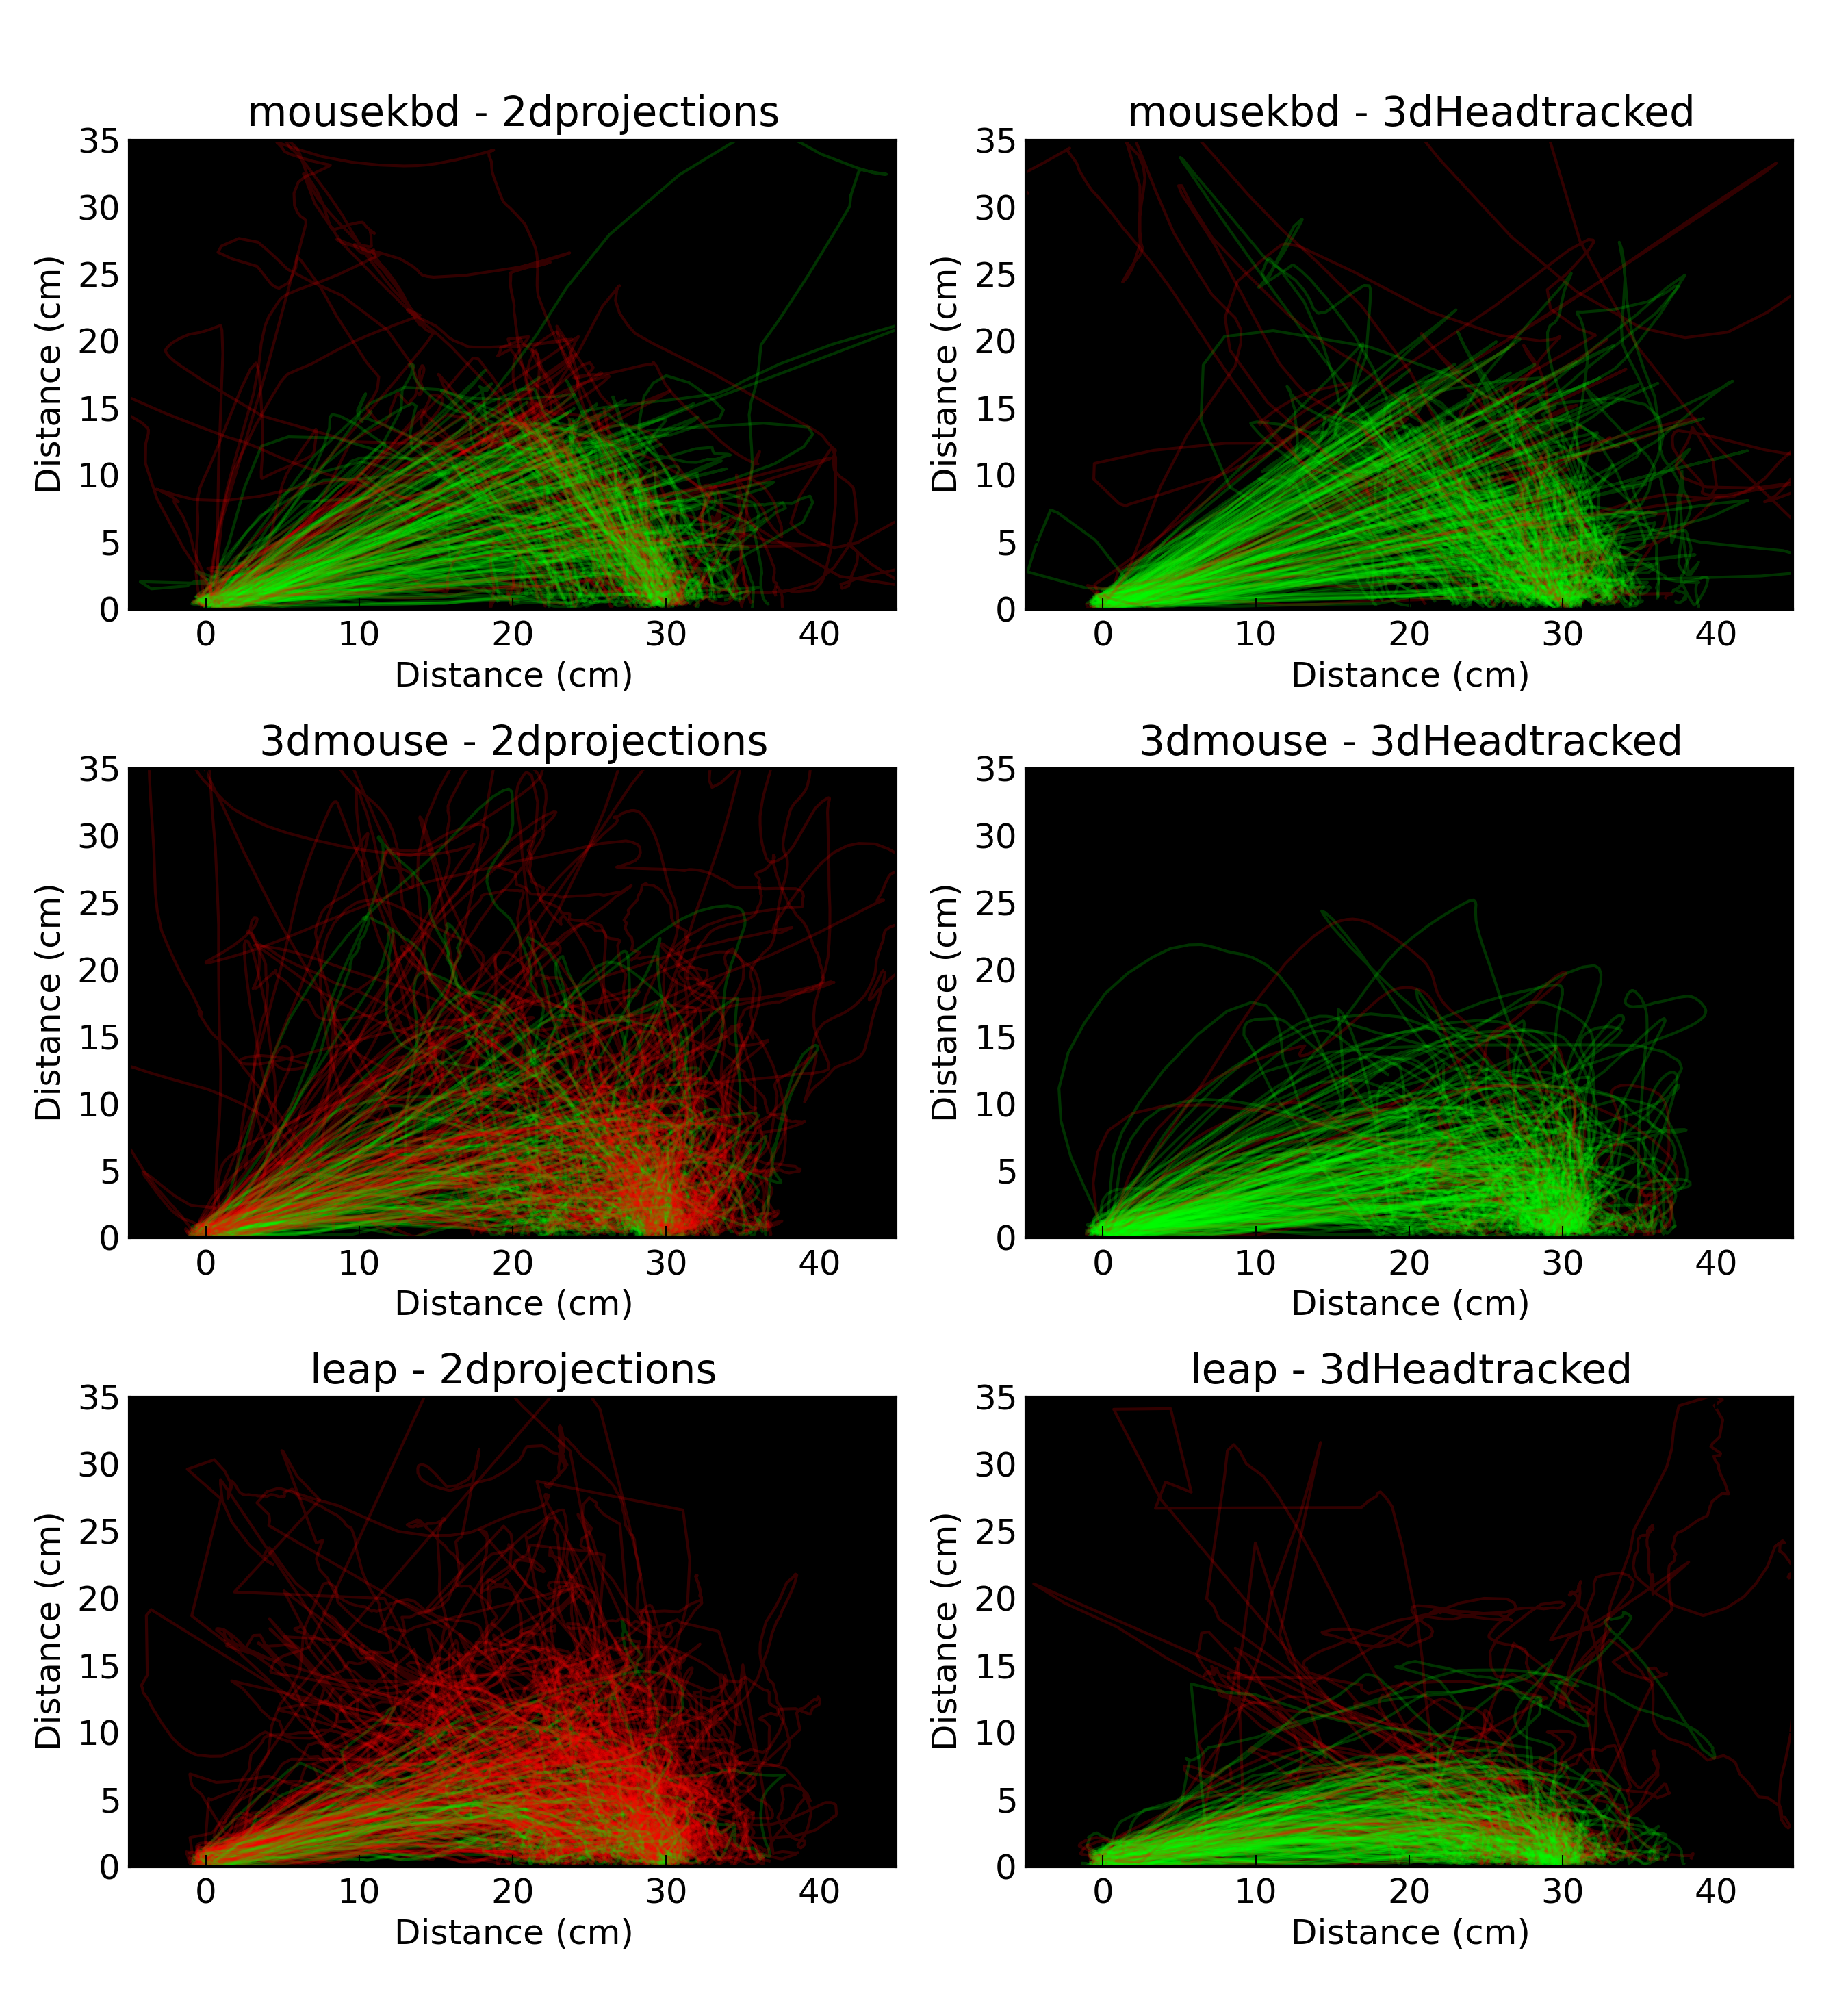
\includegraphics[width=\columnwidth]{paths.png}
    \caption{Cylinder compressed tracks}
    \label{fig:compressedtracks}
\end{figure}

We can see that subjects adopted similar strategies for the mouse and keyboard
regardless of the display type: straight line movements in orthogonal planes.
Orthogonality can't be avoided, but this shows that skills developed in
traditional 2D displays readily transfer.  That is, though the mouse is a
relative positioning input device, users have learned good mouse-eye
coordination that allows them to quickly reposition the cursor on a plane
using mostly straight line motions.

The straight-line orthogonal movement strategy is also somewhat evident for
the 3D mouse and Leap in the 2D projection case, but their tracks are still
quite organic looking.  From observing the subjects we noticed that,
especially for the 3D mouse, 3D inputs in the 2D projection case were
unintuitive for most subjects, but that after even the 20 trials conducted,
they were able to learn a decent mapping from hand motion to cursor motion.
See for example \figref{improvementtimes}.

\figref{improvementtimes} which shows the average reduction in completion time
between the first 3 trials of 20 for an input/output combination, and the last
3.  We interpret a small reduction as meaning not much learning had to take
place to saturate proficiency, whereas a large reduction is indicative of an
unintuitive input modality.  For example, subjects did not tend to get much
better using the mouse and keyboard irrespective of output type, but they did
improve quite a bit on the 3D mouse in the 2D projections case (unintuitive).
Likewise, the Leap in 3D seems to be quite intuitive as the improvement was
slight and with low variance.

\begin{figure}
    \centering

    \begin{tabular}{l | c c c}
      $ $             & MouseKbd       & 3D Mouse       & Leap          \\
      \hline
      2D Projections  & -0.199 (0.466)  & -0.892 (1.281)  & -0.204 (2.104) \\
      3D Headtracked  & -0.234 (0.729)  & -0.130 (0.485)  & -0.079 (0.336) \\
    \end{tabular}
   
    \caption{Learning the inputs, reduction in completion time in (s).  Mean (Std Dev).}
    \label{fig:improvementtimes}
\end{figure}
